% COMPOSITE

\newpage

\subsection{Problem 5}

The figure below shows vectors $\vec{A}$ and $\vec{B}$.

\begin{center}
	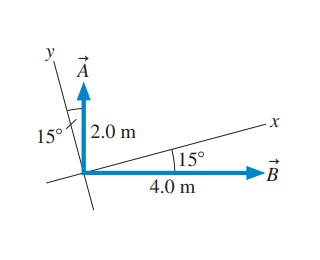
\includegraphics[width=0.5\textwidth]{/Users/max/course-manager/data/semester/Spring 2025/course/PHY2111/chapter/Vectors and Coordinate Systems/section/Quiz/figures/figure_2.jpg}
\end{center}

\setcounter{partcounter}{1}
\paragraph{Part A}

Find $\vec{D} = 4.70 \vec{A} + \vec{B}$. Express components of $\vec{D}$ in meters and separated by a comma.

\begin{solution}
	First, we will find the components of $\vec{A}$ and $\vec{B}$ relative to the Cartesian plane.
	\begin{align*}
		\vec{A}_{\mathrm{\theta}} &= \SI{90}{\degree} - \SI{15}{\degree} = \SI{75}{\degree} \\
		\vec{A}_{x} &= \SI{2.0}{m} \cos \left( \SI{75}{\degree} \right) \\
		\vec{A}_{y} &= \SI{2.0}{m} \sin \left( \SI{75}{\degree} \right)
		.\end{align*}
	\begin{align*}
		\vec{B}_{x} &= \SI{4.0}{m} \cos \left( \SI{-15}{\degree} \right) \\
		\vec{B}_{y} &= \SI{4.0}{m} \sin \left( \SI{-15}{\degree} \right)
		.\end{align*}
	Then,
	\begin{align*}
		4.70 \vec{A} &= 4.70 \left( \SI{2.0}{m} \cos \left( \SI{75}{\degree} \right), \SI{2.0}{m} \sin \left( \SI{75}{\degree} \right) \right) \\
		&= \left( \SI{2.43}{m}, \SI{9.08}{m} \right)
		.\end{align*}
	\begin{align*}
		&\left( \SI{2.43}{m}, \SI{9.08}{m} \right) + \left( \SI{4.0}{m} \cos \left( \SI{-15}{\degree} \right), \SI{4.0}{m} \sin \left( \SI{-15}{\degree} \right) \right) \\
		&= \left( \SI{6.297}{m}, \SI{8.044}{m} \right)
		.\end{align*}
\end{solution}
